\documentclass{article}
\usepackage{tikz}
\usetikzlibrary{arrows.meta}

\begin{document}

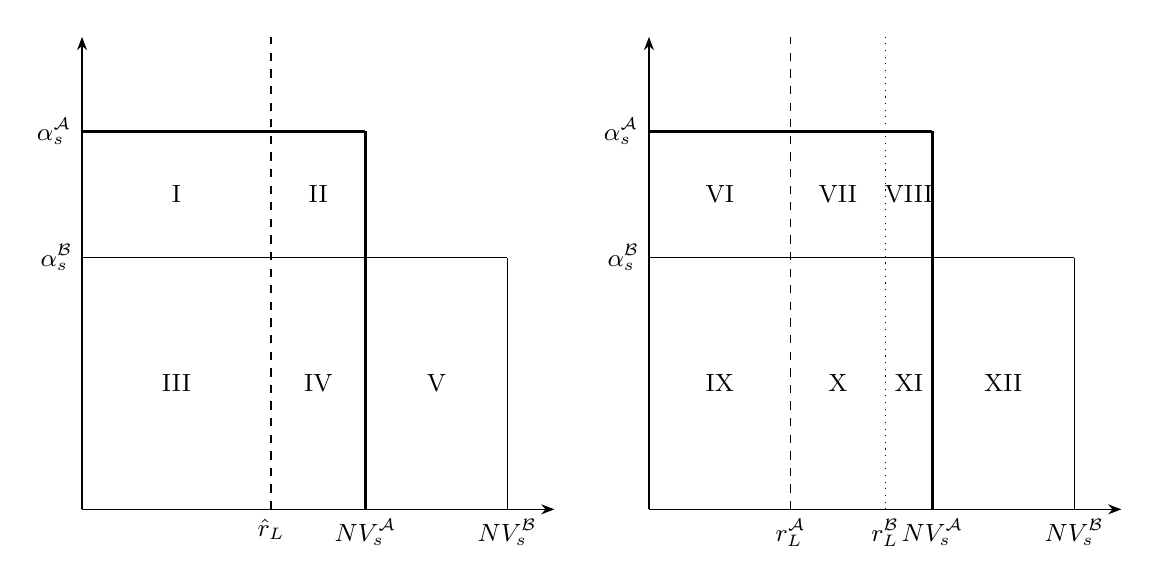
\begin{tikzpicture}[
    scale=1.2,
    every node/.style={font=\small},
    axis/.style={-Stealth},
    dashedline/.style={dashed},
    dottedline/.style={dotted},
    solidline/.style={solid}
]

% Left plot
\begin{scope}[xshift=0cm]
    % Axes
    \draw[axis] (0,0) -- (5,0);
    \draw[axis] (0,0) -- (0,5) node[left] {};
    \draw[line width=1.2pt] (0,4) node[left] {$\alpha_s^{\mathcal A}$} -- (3,4);
    \draw (0,2.665) node[left] {$\alpha_s^{\mathcal B}$} -- (4.5,2.665);
    \draw[line width=1.2pt] (3,0) -- (3,4);
    \draw (4.5,0) -- (4.5,2.665);
    \draw[dashedline] (2,0) -- (2,5);
    
    % Labels on x-axis
    \node[below] at (2,0) {$\hat{r}_L$};
    \node[below] at (3,0) {$NV^{\mathcal A}_s$};
    \node[below] at (4.5,0) {$NV^{\mathcal B}_s$};
    
    % Region labels
    \node at (1,3.3325) {I};
    \node at (2.5,3.3325) {II};
    \node at (1,1.3325) {III};
    \node at (2.5,1.3325) {IV};
    \node at (3.75,1.3325) {V};
\end{scope}

% Right plot
\begin{scope}[xshift=6cm]
    % Axes
    \draw[axis] (0,0) -- (5,0);
    \draw[axis] (0,0) -- (0,5) node[left] {};
    \draw[line width=1.2pt] (0,4) node[left] {$\alpha_s^{\mathcal A}$} -- (3,4);
    \draw (0,2.665) node[left] {$\alpha_s^{\mathcal B}$} -- (4.5,2.665);
    \draw[line width=1.2pt] (3,0) -- (3,4);
    \draw (4.5,0) -- (4.5,2.665);
    \draw[dashedline] (1.5,0) -- (1.5,5);
    \draw[dottedline] (2.5,0) -- (2.5,5);
    
    % Labels on x-axis
    \node[below] at (1.5,0) {$r_L^{\mathcal A}$};
    \node[below] at (2.5,0) {$r_L^{\mathcal B}$};
    \node[below] at (3,0) {$NV^{\mathcal A}_s$};
    \node[below] at (4.5,0) {$NV^{\mathcal B}_s$};
    
    % Region labels
    \node at (0.75,3.3325) {VI};
    \node at (2,3.3325) {VII};
    \node at (2.75,3.3325) {VIII};
    \node at (0.75,1.3325) {IX};
    \node at (2,1.3325) {X};
    \node at (2.75,1.3325) {XI};
    \node at (3.75,1.3325) {XII};
\end{scope}

\end{tikzpicture}

\end{document}
